% XXX discuss the spill-in efficiency etc.

\documentclass[../thesis.tex]{subfiles}

\begin{document}

\chapter{Oscillation fit}
\label{chap:fitting}

\section{Introduction}
\label{sec:fittingIntro}

At this stage in the analysis, we have a sample of IBD candidates, the background predictions, and the calculated efficiency corrections (for the muon veto and the multipliticy cut). The next step is to take the background-subtracted and efficiency-corrected IBD prompt spectra at the eight ADs, and fit them to the 3-flavor oscillation model in order to extract $\SinSq$ and $\Dmsqee$.

Our analysis is based on the Daya Bay oscillation fitter developed at Lawrence Berkeley National Laboratory (LBNL) \cite{berkeley_shapefit,berkeley_toymc}, which is one of a half-dozen independent fitters used in the production and cross-checking of Daya Bay's official oscillation fits. While it is relatively straightforward to find the oscillation parameters that best fit Daya Bay's data, determining their uncertainties is significant more complicated, given the need to consider a wide range of systematics (e.g., those related to the reactors, the detectors, and the backgrounds). The modeling and methods used by the LBNL fitter have been carefully developed and validated over the years, allowing our analysis to benefit from these efforts. Furthermore, our use of the LBNL fitter ensures that our cut-variation studies are directly applicable to Daya Bay's past and future results.

The LBNL fitter is a \emph{relative} fitter: That is, instead of simultaneously comparing all eight ADs to a model of the reactor spectra and oscillation probability (an \emph{absolute} fit), it uses the measurements of the near ADs to predict the far AD spectra (including oscillation effects). This approach ensures that the results are independent (to first-order) of the modeling used for the reactor spectra. A reactor model is still required in order to decompose each near AD's spectrum into the components from individual cores, but the final result is negligibly affected by the details of the model. Among the Daya Bay fitters developed outside of LBNL, some take the absolute approach, and they too are able to produce results that are stable across reactor models, but this requires using explicit nuisance parameters (or ``pull terms'') to represent the uncertainties in the reactor modeling.

Aside from its use of a relative approach, a second defining characterstic of the LBNL fitter is its use of a covariance matrix to encode all systematic (as well as statistical) uncertainties. This ensures that finding the best-fit oscillation parameters is a simple two-dimensional minimization problem, with an objective function of the form
\begin{equation}
  \label{eq:fitChiSqOverview}
  \chi^2 = (F_i - \widebar F_i) V_{ij}^{-1} (F_j - \widebar F_j).
\end{equation}
where the index $i$ runs over the energy bins in the far hall, the $F_i$ are the measured far-hall spectra, the $\widebar F_i$ are the predicted far-hall spectra based on the near-hall observations, and $V_{ij}$ is the total covariance matrix (including both systematic and statistical components). All of the complexity lies in the determination of $V_{ij}$ (which we discuss shortly). In contrast to the covariance matrix approach, it is possible to parameterize each systematic with a pull term $\eta_j$ (and a corresponding nominal value $\widebar \eta_j$ and variance $\zeta_j^2$), resulting in an objective function akin to
\begin{equation}
  \chi^2 = \sum_i \frac{(F_i - \widebar F_i)^2}{\sigma_i^2} + \sum_j \frac{(\eta_j - \widebar \eta_j)^2}{\varsigma_j^2}.
\end{equation}
In this case, the predictions $\widebar F_i$ are implicitly dependent on the pull terms $\eta_j$. Performing the fit then involves finding both the oscillation parameters \emph{and the pull terms} that minimize $\chi^2$. This is a high-dimensional minimization problem, with an attendant computational cost and need to avoid false minima, but it avoids the calculation of a complex covariance matrix. Both methods, covariance-matrix-based and pull-term-based, can be used in either a relative or an absolute approach, leading to a total of four options. Each option has benefits and drawbacks from the standpoint of implementation complexity; however, assuming the use of consistent modeling, all four should give consistent final results, as has indeed been demonstrated repeatedly during the Collaboration's internal cross-checks. We do not make any claim of superiority for the LBNL fitter's relative, covariance-matrix approach; it is simply what we have chosen to use. Further discussion of these different methodologies can be found in \autoref{sec:fitoverview}.

As was mentioned, the price of a simple two-dimensional minimization is that we must first calculate the covariance matrix $V_{ij}$. This matrix encodes the variance in each energy bin, and its covariances with other bins, as the combination of contributions from \emph{all} sources of uncertainty, systematic and statistical. For any reasonably complex experiment such as Daya Bay, this cannot be done analytically, or even (deterministically) numerically. Instead, Monte Carlo (MC) must be used. The LBNL fitter includes a toy MC for this purpose. The toy MC generates sets of predicted prompt spectra at the eight ADs. Each set (``toy sample'') is generated under randomized assumptions regarding detector and background uncertainties. From a large ensemble of toy samples, the covariance between each pair of energy bins can be calculated, giving a partial covariance matrix that accounts only for the detector and background systematics. This is then combined with two other matrices: a preexisting covariance matrix that accounts for reactor-related systematics, and an analytically calculated statistical covariance matrix, giving the full matrix used in this fit.

In the remainder of this chapter, we provide basic overviews of the reactor model, the toy MC, and the fitter, as well as a summary of our inputs and results. Further details can be found in Appendices~\ref{chap:reactor} and \ref{chap:fittingDetails}.

\section{Reactor model}
\label{sec:fittingReactor}

Although the details of the reactor model have minimal bearing on the final result, a model must still be chosen in order to decompose each near AD's spectra into individual reactor contributions, for extrapolation to the far hall. In keeping with the official practice of the Collaboration, we use the results of Huber \cite{PhysRevC.84.024617} and Mueller \cite{PhysRevC.83.054615}. In particular, for fissions of $^{235}$U, $^{239}$Pu, and $^{241}$Pu, we use Huber's conversions of the total $\beta$ spectra measured at Institut Laue-Langevin (ILL), while for $^{238}$U, we use Mueller's \emph{ab initio} calculations based on nuclear data. These predictions include time-dependent corrections for each reactor's departure from equilibrium, as well as additional contributions from the spent nuclear fuel (SNF) pools near each core.

The four individual isotope spectra must then be appropriately scaled and combined to obtain the total prediction for each core. This is accomplished using data provided by the power plant on each core's weekly average power and fission fractions. This allows the total nominal spectrum $\Phi^0_{c,t}(E_\nu)$ (per unit time) at each core $c$ to be determined, for week $t$, as:
\begin{equation}
  \Phi^0_{c,t}(E_\nu) = \sum_k \left( \frac{W_{c,t}) \, f_{k,t}}{\sum_k f_{k,t} \, e_k}
    S_k(E) \, c^{\mathrm{ne}}_{k,t}(E) \right) + S^{\mathrm{snf}}_t(E),
\end{equation}
where the index $k$ runs over the four fission isotopes, $W_t$ is the average thermal power, the $f_{k,t}$ are the fission fractions, the $e_k$ are the average energy released per fission, the $S_k(E)$ are the Huber-Mueller isotope spectra, the $c^{\mathrm{ne}}_{k,t}(E)$ are the off-equilibrium corrections, and $S^{\mathrm{snf}}_t(E)$ is the SNF contribution.

Livetime-weighted summing of these weekly spectra then gives the predictions for the entire data period:
\begin{equation}
  \Phi^0_c(E_\nu) = \frac{\sum_t T_t \Phi^0_{c,t}(E_\nu)}{\sum_t T_t},
\end{equation}
where the $T_t$ are the weekly livetimes. The toy MC can then feed these spectra into its model of propagation/oscillation, the IBD cross-section, and the detector response, producing a toy sample of the predicted prompt spectrum at each AD.

Aside from the predicted core spectra, the reactor model is also responsible for producing the reactor-related covariance matrix. This is done by quantifying all systematic uncertainties, include those on the weekly power, the fission fractions, the isotope spectra, and the off-equilibrium correction \cite{Lewis}. The model is then used to generate samples of core spectra under variations of these systematics. Letting $\Phi_{a}$ denote the vector containing the binned spectra from all the cores (such that the index $a$ runs over bins and cores), the reactor covariance matrix $V^{\mathrm{reac}}$ is
\begin{equation}
  V^{\mathrm{reac}}_{ab} = \frac{1}{M} \sum_{n=1}^M(\Phi^n_{a} - \Phi^0_{a})(\Phi^n_{b} - \Phi^0_{b}),
\end{equation}
where the index $n$ runs over the $M$ simulated spectra. The Cholesky decomposition $U$ of $V^{\mathrm{reac}}$, where
\begin{equation}
  V^{\mathrm{reac}} = U^TU,
\end{equation}
is later used by the LBNL toy MC to generate a fluctuated core spectrum for each toy sample:
\begin{equation}
  \label{eq:fitCholeskyUsage}
  \Phi_c(E_\nu) = \Phi^0_c(E_\nu) + \sum_b U_{a_c(E_\nu)b} y_b,
\end{equation}
where $a_c(E_\nu)$ is the index corresponding to core $c$ and energy $E_\nu$, $b$ runs over all cores and energy bins, and $y_b$ is a vector of standard normal random variables.

\section{Toy Monte Carlo}
\label{sec:fittingToyMC}

Given the livetime-normalized antineutrino spectrum $\Phi_c(E_\nu)$ at each core $c$ (including any random fluctuations applied using $V^{\mathrm{reac}}$), the LBNL toy MC begins by calculating the antineutrino spectrum $R_i(E_\nu)$ at each AD $i$:
\begin{equation}
  \label{eq:fitTrueIbdSpecOverview}
  R_i(E_\nu) = T_i\,N_i\,\epsilon_i\,\sigma(E_\nu) \sum_c F_c(E_\nu) \frac{1}{4\pi L_{ci}^2}
  \Posc(E_\nu, L_{ci}),
\end{equation}
where $T_i$ is the livetime, $N_i$ is the number of target protons, $L_{ci}$ is the baseline, $\epsilon_i$ is the detection efficiency (comprising the muon-veto and multiplicity-cut efficiencies), and $\sigma(E_\nu)$ is the IBD cross-section (\autoref{eq:ibdXsec}). $\Posc$ depends on the assumption of nominal oscillation parameters; however, the final result is stable against reasonable variations in these assumptions. The $R_i$ may be freely multiplied by a common constant factor without affecting the oscillation fit; as such, the efficiency $\epsilon_i$ does not account for factors that are equal among all ADs. Similarly, there is no impact from any constant error in the absolute normalization of the core spectra. It is only necessary that the $R_i$ correctly capture the \emph{relative} rates and shapes between the ADs.

The antineutrino spectra $R_i(E_\nu)$ must be converted by the toy MC into reconstructed prompt-energy spectra. The first step in this process is to convert antineutrino energy $E_\nu$ into positron energy (including rest mass) $E_e$ using \autoref{eq:firstOrderEnergyMean}. Next, a detector response matrix (\autoref{sec:fitIavEffect}) is used to convert $E_e$ into the total \emph{scintillator-deposited} energy $E_{\mathrm{dep}}$, which accounts for energy loss in the acrylic. $E_{\mathrm{dep}}$ is then converted to the average corresponding reconstructed energy using the detector nonlinearity model (\autoref{sec:fitEeToMeanErec}). Finally, the reconstructed energy is smeared using the detector resolution model (\autoref{sec:fitResolution}). These various aspects of the detector response model can be randomly fluctuated during the generation of each toy sample.

The final step in generating each toy sample is to add backgrounds to the prompt spectra. This is accomplished trivially, by taking the nominal shape of each background, scaling it according to the predicted rate, and adding it to the IBD prompt spectrum. Both the rate and the shape can be fluctuated in accordance with the background uncertainties (\autoref{sec:fitToyBackgrounds}).

In practice, we generate two sets of toy samples, corresponding to signal-related (i.e., reactor and detector) and background-related fluctuations, respectively. The former matrix is proportional to the toy MC's assumptions on the absolute normalization (reactor flux and detection efficiency); it should thus be rescaled according to the measured normalization (\autoref{sec:fitToyCovMatDetails}). Meanwhile, the backgrounds are insensitive to the flux normalization, and their data-driven estimations already account for the detection efficiency, so no rescaling is necessary for the background matrix. Since the two are treated differently, they must be generated separately, from separate sets of toy samples.

\def\Fbar{\widebar F}

Before presenting the calculation of the covariance matrices, we must pause to discuss the binning scheme employed. As was explained, the LBNL fitter compares the far-site data to the far-site predictions obtained from the near-site data. In practice, as discussed in \autoref{sec:fitCombo}, we combine the data from all the ADs in a given hall, and we consider \emph{two} predictions for EH3: one from EH1, and one from EH2. These predictions are further divided among 37 energy bins (\autoref{sec:binning}) and three time bins (the 6, 8, and 7-AD periods), giving a total of
\begin{equation}
  2 \times 37 \times 3 = 222
\end{equation}
predictions, which we represent by the vector $\Fbar_i$, where the index $i$ runs over the 222 individual predictions. Meanwhile, the number of far-site \emph{observations} is equal to 111, half of the number of predictions, since we have separate predictions from EH1 and EH2. We represent the background-subtracted and efficiency-corrected observations in the vector $F_i$, in which each observation is repeated twice, in alignment with $\Fbar_i$. 

Given $M$ toy samples, indexed by the variable $t$, the background covariance matrix $V_{\mathrm{bkg}}$ is calculated according to
\begin{equation}
  (V_{\mathrm{bkg}})_{ij} = \frac{1}{M} \sum_t^{M}
  (F_i - \Fbar_i)(F_j - \Fbar_j).
\end{equation}
The signal covariance matrix $V_{\mathrm{sig}}$, on the other hand, must be rescaled to account for the measured absolute normalization:
\begin{equation}
  (V_{\mathrm{sig}})_{ij} = \frac{1}{M} \sum_t^M
  \frac{F_i \cdot F_j}{\Fbar_i \cdot \Fbar_j}
  (F_i - \Fbar_i)(F_j - \Fbar_j)}.
\end{equation}

The statistical covariance matrix $V_{\mathrm{stat}}$ is not calculated from the toy samples, but rather from the measured data. As discussed in \autoref{sec:fitStatCovMat}, for a given prediction-bin $i$, the corresponding diagonal element of $V_{\mathrm{stat}}$ is
\begin{equation}
  (V_{\mathrm{stat}})_{ii} = (\sigma_{\mathrm{near}})_{i}^2 + (\sigma_{\mathrm{far}})_{i}^2,
\end{equation}
where
\begin{equation}
  \begin{aligned}
    (\sigma_{\mathrm{near}})_i &= \frac{\Fbar_i}{N_i} \sqrt{N_i + N_i^{\mathrm{bkg}}}\\
    (\sigma_{\mathrm{far}})_i &= \sqrt{\Fbar_i} + F_i^{\mathrm{bkg}}}.
  \end{aligned}
\end{equation}
Here, $N$ is the (background-subtracted) near-site observation, $N^{\mathrm{bkg}}$ is the expected near-site background, and $F^{\mathrm{bkg}}$ is the far-site background. Given our method of binning and combining the data, an off-diagonal element $(V_{\mathrm{stat}})_{ij}$ is nonzero only when $i$ and $j$ correspond to the same far-site energy bin and data period, differing only when it comes to the near-site used for the prediction. More precisely,
\begin{equation}
  \left. (V_{\mathrm{stat}})_{ij} \right|_{i \ne j} = K_{ij} (\sigma_{\mathrm{far}})_i (\sigma_{\mathrm{far}})_j,
\end{equation}
where $K_{ij} = 1$ if prediction-bins $i$ and $j$ correspond to the same far-site observation, and zero otherwise.

The total covariance matrix $V$ is then calculated as the sum of the three above:
\begin{equation}
  V = V_{\mathrm{sig}} + V_{\mathrm{bkg}} + V_{\mathrm{stat}}.
\end{equation}

\section{Fitter}
\label{sec:fitFitterOverview}

Compared to the toy MC, whose main purpose is to generate the covariance matrix $V$, the fitter's role is to find the oscillation parameters that minimize the $\chi^2$ given by \autoref{eq:fitChiSqOverview}. Most of the fitter's complexity comes not from the minimization procedure, which is conducted using the well-established numerical library MINUIT. Rather, the complexity arises from the calculation of the far-site predictions $\Fbar_i$. As illustrated in \autoref{fig:fitExtrapCartoonOverview}, this process involves using reactor knowledge (and a given set of oscillation parameters) to decompose each near-site observation into the sum of components from individual cores. Each component is then separately extrapolated to the far site, accounting for the difference in baselines. The components are then summed to give the prediction $\Fbar_i$. The technical details of this procedure can be found in \autoref{sec:fitNearToFarPred}.

\begin{figure}[ht!]
  \centering
  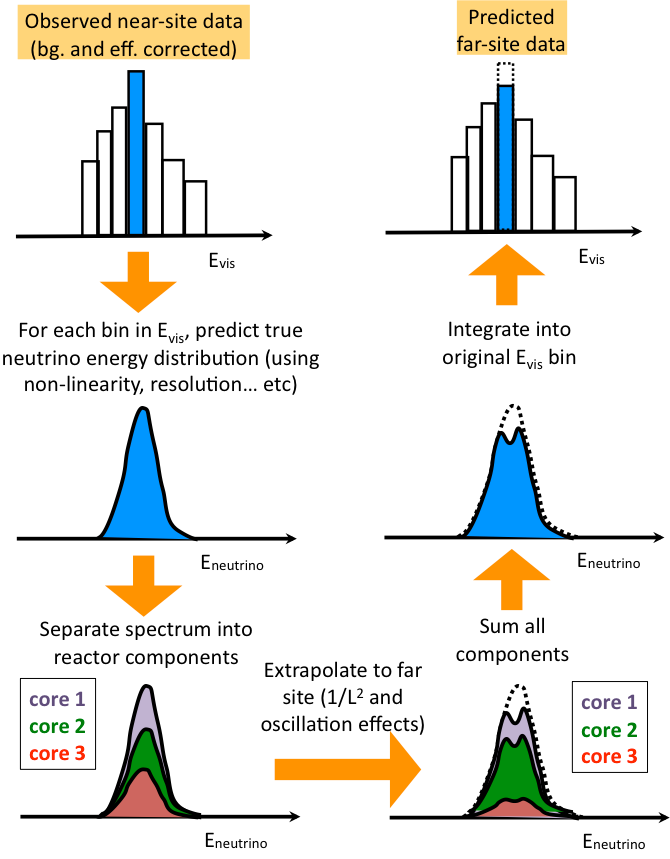
\includegraphics[scale=0.5]{extrap_cartoon.png}
  \caption{Conceptual illustration of the procedure for extrapolating a near AD measurement to a far AD. In the bottom-right panel, the dashed curve represents the unoscillated prediction. From \cite{berkeley_shapefit}.}
  \label{fig:fitExtrapCartoonOverview} 
\end{figure}

Given the observations $F_i$, the covariance matrix $V_{ij}$, and the ability to calculate $\Fbar_i$ as a function of the oscillation parameters, the remainder of the fit procedure is straightforward. We provide $\chi^2(\SinSq, \Dmsqee)$ (\autoref{eq:fitChiSqOverview}) to the minimization library, which then returns the best-fit values of the oscillation parameters. Beyond reporting the best-fit parameters, the fitter also generates a grid of $\chi^2$ values in the $\SinSq$-$\Dmsqee$ parameter space, enabling the calculation of two-dimensional contours at any desired confidence level (\autoref{sec:fitContours}).

\section{Results}
\label{sec:fitResults}

\autoref{fig:fitContours} shows the results of applying the fitter to our sample of IBD candidates. For this sample, AD-specific quantities (signal and background rates, efficiencies, etc.) are summarized in Tables~\ref{tab:fitting_inputs_6ad}--\ref{tab:fitting_inputs_7ad}. We obtain the following best-fit oscillation parameters:
% From 2021_02_03@delcut_third_6.000MeV@newAcc
% Previously was using 2020_01_26@yolo2? (doc-12115)
% fit_shape_2d:
% Event: 0; --> best fit: 0.0853245,0.00246905; minchi2=216.034
% plot_contours:
% sin^2(2theta_13) = 0.0853245 - 0.00287582 + 0.00286401
% delta m^2_ee or delta m^2_32 check carefully! = 0.00246905 - 7.22585e-05 + 7.06787e-05
\begin{equation}
    \SinSq = 0.0853 \pm 0.0029 \qquad \Dmsqee = 2.47\times10^{-3} \pm 7.2\times10^{-5},
  \label{eq:fitResults}
\end{equation}
where the errors include both statistical and systematic uncertainties (as encoded and combined in the covariance matrix, \autoref{eq:fitCovmatSum}). The minimum $\chi^2$ is given by
\begin{equation}
  \chi^2 / \nu = 216.0 / 220 = 0.9818 \qquad (p = 0.564).
\end{equation}
Here, the number $\nu$ of degrees of freedom is\footnote{Recall, as discussed in \autoref{sec:fitCombo}, that we have two predictions per data period and energy bin: One prediction of EH3 from EH1, and one of EH3 from EH2, where all ADs within a given hall are combined.}
\begin{equation}
  \begin{aligned}
    \nu &= N_{\mathrm{periods}} \times N_{\mathrm{predictions}} \times N_{E\;\mathrm{bins}} - N_{\mathrm{osc\;pars}} \\
    &= 3 \times 2 \times 37 - 2 \\
    &= 220.
  \end{aligned}
\end{equation}
These oscillation parameters are consistent with those published in \cite{An_2017}. This is particularly unsurprising in light of our use of practically the same IBD selection criteria as Selection B in that publication. In \autoref{chap:cutVary}, we proceed to explore the effects of changing these criteria, with the aim of demonstrating that the result remains consistent.

% Ran dumpBigTable.jl on 2021_02_03@delcut_third_6.000MeV@newAcc

\begin{table}[ht]
  \resizebox{\textwidth}{!}{%
    \begin{tabular}{lcccccccc}
      \toprule
      &  \multicolumn{2}{c}{EH1} & \multicolumn{2}{c}{EH2} & \multicolumn{4}{c}{EH3} \\
      &  AD1 & AD2 & AD1 & AD2 & AD1 & AD2 & AD3 & AD4 \\
      \midrule
      IBD candidates &  99099 & 100547 & 91655 & \phantom{0} & 13814 & 13722 & 13554 & \phantom{0} \\
      Livetime (days) &  186.786 & 186.786 & 187.190 & \phantom{0.000} & 187.666 & 187.666 & 187.666 & \phantom{0.000} \\
      Target mass (kg) &  19941 & 19966 & 19891 & \phantom{19945} & 19913 & 19991 & 19892 & \phantom{19931} \\
      Veto eff. &  0.8163 & 0.8140 & 0.8480 & \phantom{0.0000} & 0.9808 & 0.9803 & 0.9802 & \phantom{0.0000} \\
      Mult.\ eff. &  0.9765 & 0.9768 & 0.9778 & \phantom{0.0000} & 0.9769 & 0.9767 & 0.9766 & \phantom{0.0000} \\
      Accidentals (day$^{-1}$) &  9.12 $\pm$ 0.18 & 8.89 $\pm$ 0.18 & 7.20 $\pm$ 0.14 & \phantom{0.00 $\pm$ 0.00} & 2.80 $\pm$ 0.06 & 2.76 $\pm$ 0.06 & 2.71 $\pm$ 0.05 & \phantom{0.00 $\pm$ 0.00} \\
      $^9$Li/$^8$He (day$^{-1}$) &  2.35 $\pm$ 0.64 & 2.35 $\pm$ 0.64 & 1.50 $\pm$ 0.43 & \phantom{0.00 $\pm$ 0.00} & 0.21 $\pm$ 0.08 & 0.21 $\pm$ 0.08 & 0.21 $\pm$ 0.08 & \phantom{0.00 $\pm$ 0.00} \\
      Fast neutrons (day$^{-1}$) &  0.84 $\pm$ 0.08 & 0.84 $\pm$ 0.08 & 0.64 $\pm$ 0.06 & \phantom{0.00 $\pm$ 0.00} & 0.05 $\pm$ 0.01 & 0.05 $\pm$ 0.01 & 0.05 $\pm$ 0.01 & \phantom{0.00 $\pm$ 0.00} \\
      $^{241}$AmC-$^{13}$C (day$^{-1}$) &  0.29 $\pm$ 0.13 & 0.27 $\pm$ 0.12 & 0.30 $\pm$ 0.14 & \phantom{0.00 $\pm$ 0.00} & 0.24 $\pm$ 0.11 & 0.23 $\pm$ 0.10 & 0.23 $\pm$ 0.10 & \phantom{0.00 $\pm$ 0.00} \\
      $^{13}$C($\alpha,n$)-$^{16}$O (day$^{-1}$) &  0.09 $\pm$ 0.04 & 0.07 $\pm$ 0.04 & 0.05 $\pm$ 0.02 & \phantom{0.00 $\pm$ 0.00} & 0.05 $\pm$ 0.02 & 0.04 $\pm$ 0.02 & 0.04 $\pm$ 0.02 & \phantom{0.00 $\pm$ 0.00} \\
      \midrule
      IBD rate (day$^{-1}$) &  652.91 $\pm$ 2.22 & 663.71 $\pm$ 2.24 & 582.30 $\pm$ 2.01 & \phantom{0.00 $\pm$ 0.00} & 73.58 $\pm$ 0.67 & 72.88 $\pm$ 0.67 & 72.39 $\pm$ 0.66 & \phantom{0.00 $\pm$ 0.00} \\
      \bottomrule
    \end{tabular}
  }
  \caption{Summary of inputs used in the oscillation fit (6AD period).}
  \label{tab:fitting_inputs_6ad}
\end{table}

\begin{table}[ht]
  \resizebox{\textwidth}{!}{%
    \begin{tabular}{lcccccccc}
      \toprule
      &  \multicolumn{2}{c}{EH1} & \multicolumn{2}{c}{EH2} & \multicolumn{4}{c}{EH3} \\
      &  AD1 & AD2 & AD1 & AD2 & AD1 & AD2 & AD3 & AD4 \\
      \midrule
      IBD candidates &  727648 & 737307 & 688655 & 677720 & 98495 & 98905 & 98147 & 99155 \\
      Livetime (days) &  1349.831 & 1349.831 & 1353.589 & 1353.589 & 1351.873 & 1351.873 & 1351.873 & 1351.873 \\
      Target mass (kg) &  19941 & 19966 & 19891 & 19945 & 19913 & 19991 & 19892 & 19931 \\
      Veto eff. &  0.8235 & 0.8197 & 0.8517 & 0.8502 & 0.9832 & 0.9830 & 0.9829 & 0.9831 \\
      Mult.\ eff. &  0.9770 & 0.9769 & 0.9783 & 0.9781 & 0.9786 & 0.9787 & 0.9785 & 0.9784 \\
      Accidentals (day$^{-1}$) &  7.64 $\pm$ 0.15 & 7.55 $\pm$ 0.15 & 5.56 $\pm$ 0.11 & 5.61 $\pm$ 0.11 & 0.82 $\pm$ 0.02 & 0.76 $\pm$ 0.02 & 0.78 $\pm$ 0.02 & 0.84 $\pm$ 0.02 \\
      $^9$Li/$^8$He (day$^{-1}$) &  2.35 $\pm$ 0.64 & 2.35 $\pm$ 0.64 & 1.50 $\pm$ 0.43 & 1.50 $\pm$ 0.43 & 0.21 $\pm$ 0.08 & 0.21 $\pm$ 0.08 & 0.21 $\pm$ 0.08 & 0.21 $\pm$ 0.08 \\
      Fast neutrons (day$^{-1}$) &  0.84 $\pm$ 0.08 & 0.84 $\pm$ 0.08 & 0.64 $\pm$ 0.06 & 0.64 $\pm$ 0.06 & 0.05 $\pm$ 0.01 & 0.05 $\pm$ 0.01 & 0.05 $\pm$ 0.01 & 0.05 $\pm$ 0.01 \\
      $^{241}$AmC-$^{13}$C (day$^{-1}$) &  0.15 $\pm$ 0.07 & 0.15 $\pm$ 0.07 & 0.12 $\pm$ 0.06 & 0.14 $\pm$ 0.06 & 0.04 $\pm$ 0.02 & 0.03 $\pm$ 0.01 & 0.03 $\pm$ 0.02 & 0.04 $\pm$ 0.02 \\
      $^{13}$C($\alpha,n$)-$^{16}$O (day$^{-1}$) &  0.08 $\pm$ 0.04 & 0.06 $\pm$ 0.03 & 0.04 $\pm$ 0.02 & 0.06 $\pm$ 0.03 & 0.04 $\pm$ 0.02 & 0.04 $\pm$ 0.02 & 0.03 $\pm$ 0.02 & 0.04 $\pm$ 0.02 \\
      \midrule
      IBD rate (day$^{-1}$) &  658.93 $\pm$ 1.03 & 670.29 $\pm$ 1.03 & 604.30 $\pm$ 0.87 & 594.01 $\pm$ 0.86 & 74.67 $\pm$ 0.26 & 74.77 $\pm$ 0.26 & 74.57 $\pm$ 0.26 & 75.11 $\pm$ 0.26 \\
      \bottomrule
    \end{tabular}
  }
  \caption{Summary of inputs used in the oscillation fit (8AD period).}
  \label{tab:fitting_inputs_8ad}
\end{table}

\begin{table}[ht]
  \resizebox{\textwidth}{!}{%
    \begin{tabular}{lcccccccc}
      \toprule
      &  \multicolumn{2}{c}{EH1} & \multicolumn{2}{c}{EH2} & \multicolumn{4}{c}{EH3} \\
      &  AD1 & AD2 & AD1 & AD2 & AD1 & AD2 & AD3 & AD4 \\
      \midrule
      IBD candidates &  \phantom{0} & 122645 & 102357 & 100994 & 14894 & 15083 & 14987 & 14927 \\
      Livetime (days) &  \phantom{0.000} & 200.995 & 200.440 & 200.440 & 200.071 & 200.071 & 200.071 & 200.071 \\
      Target mass (kg) &  \phantom{19941} & 19966 & 19891 & 19945 & 19913 & 19991 & 19892 & 19931 \\
      Veto eff. &  \phantom{0.0000} & 0.8218 & 0.8550 & 0.8532 & 0.9849 & 0.9847 & 0.9846 & 0.9848 \\
      Mult.\ eff. &  \phantom{0.0000} & 0.9740 & 0.9785 & 0.9783 & 0.9787 & 0.9787 & 0.9788 & 0.9785 \\
      Accidentals (day$^{-1}$) &  \phantom{0.00 $\pm$ 0.00} & 7.26 $\pm$ 0.15 & 5.26 $\pm$ 0.11 & 5.10 $\pm$ 0.10 & 0.63 $\pm$ 0.01 & 0.64 $\pm$ 0.01 & 0.69 $\pm$ 0.01 & 0.61 $\pm$ 0.01 \\
      $^9$Li/$^8$He (day$^{-1}$) &  \phantom{0.00 $\pm$ 0.00} & 2.35 $\pm$ 0.64 & 1.50 $\pm$ 0.43 & 1.50 $\pm$ 0.43 & 0.21 $\pm$ 0.08 & 0.21 $\pm$ 0.08 & 0.21 $\pm$ 0.08 & 0.21 $\pm$ 0.08 \\
      Fast neutrons (day$^{-1}$) &  \phantom{0.00 $\pm$ 0.00} & 0.84 $\pm$ 0.08 & 0.64 $\pm$ 0.06 & 0.64 $\pm$ 0.06 & 0.05 $\pm$ 0.01 & 0.05 $\pm$ 0.01 & 0.05 $\pm$ 0.01 & 0.05 $\pm$ 0.01 \\
      $^{241}$AmC-$^{13}$C (day$^{-1}$) &  \phantom{0.00 $\pm$ 0.00} & 0.11 $\pm$ 0.05 & 0.09 $\pm$ 0.04 & 0.08 $\pm$ 0.04 & 0.02 $\pm$ 0.01 & 0.02 $\pm$ 0.01 & 0.03 $\pm$ 0.01 & 0.02 $\pm$ 0.01 \\
      $^{13}$C($\alpha,n$)-$^{16}$O (day$^{-1}$) &  \phantom{0.00 $\pm$ 0.00} & 0.05 $\pm$ 0.03 & 0.03 $\pm$ 0.02 & 0.06 $\pm$ 0.03 & 0.03 $\pm$ 0.02 & 0.03 $\pm$ 0.02 & 0.03 $\pm$ 0.01 & 0.03 $\pm$ 0.02 \\
      \midrule
      IBD rate (day$^{-1}$) &  \phantom{0.00 $\pm$ 0.00} & 750.78 $\pm$ 2.27 & 604.44 $\pm$ 1.97 & 596.17 $\pm$ 1.95 & 76.40 $\pm$ 0.64 & 77.07 $\pm$ 0.64 & 76.91 $\pm$ 0.64 & 76.54 $\pm$ 0.64 \\
      \bottomrule
    \end{tabular}
  }
  \caption{Summary of inputs used in the oscillation fit (7AD period).}
  \label{tab:fitting_inputs_7ad}
\end{table}

% Ran plot_contours.C on 2021_02_03@delcut_third_6.000MeV@newAcc
% Previously was using 2020_01_26@yolo2? (doc-12115)
\begin{figure}[ht]
  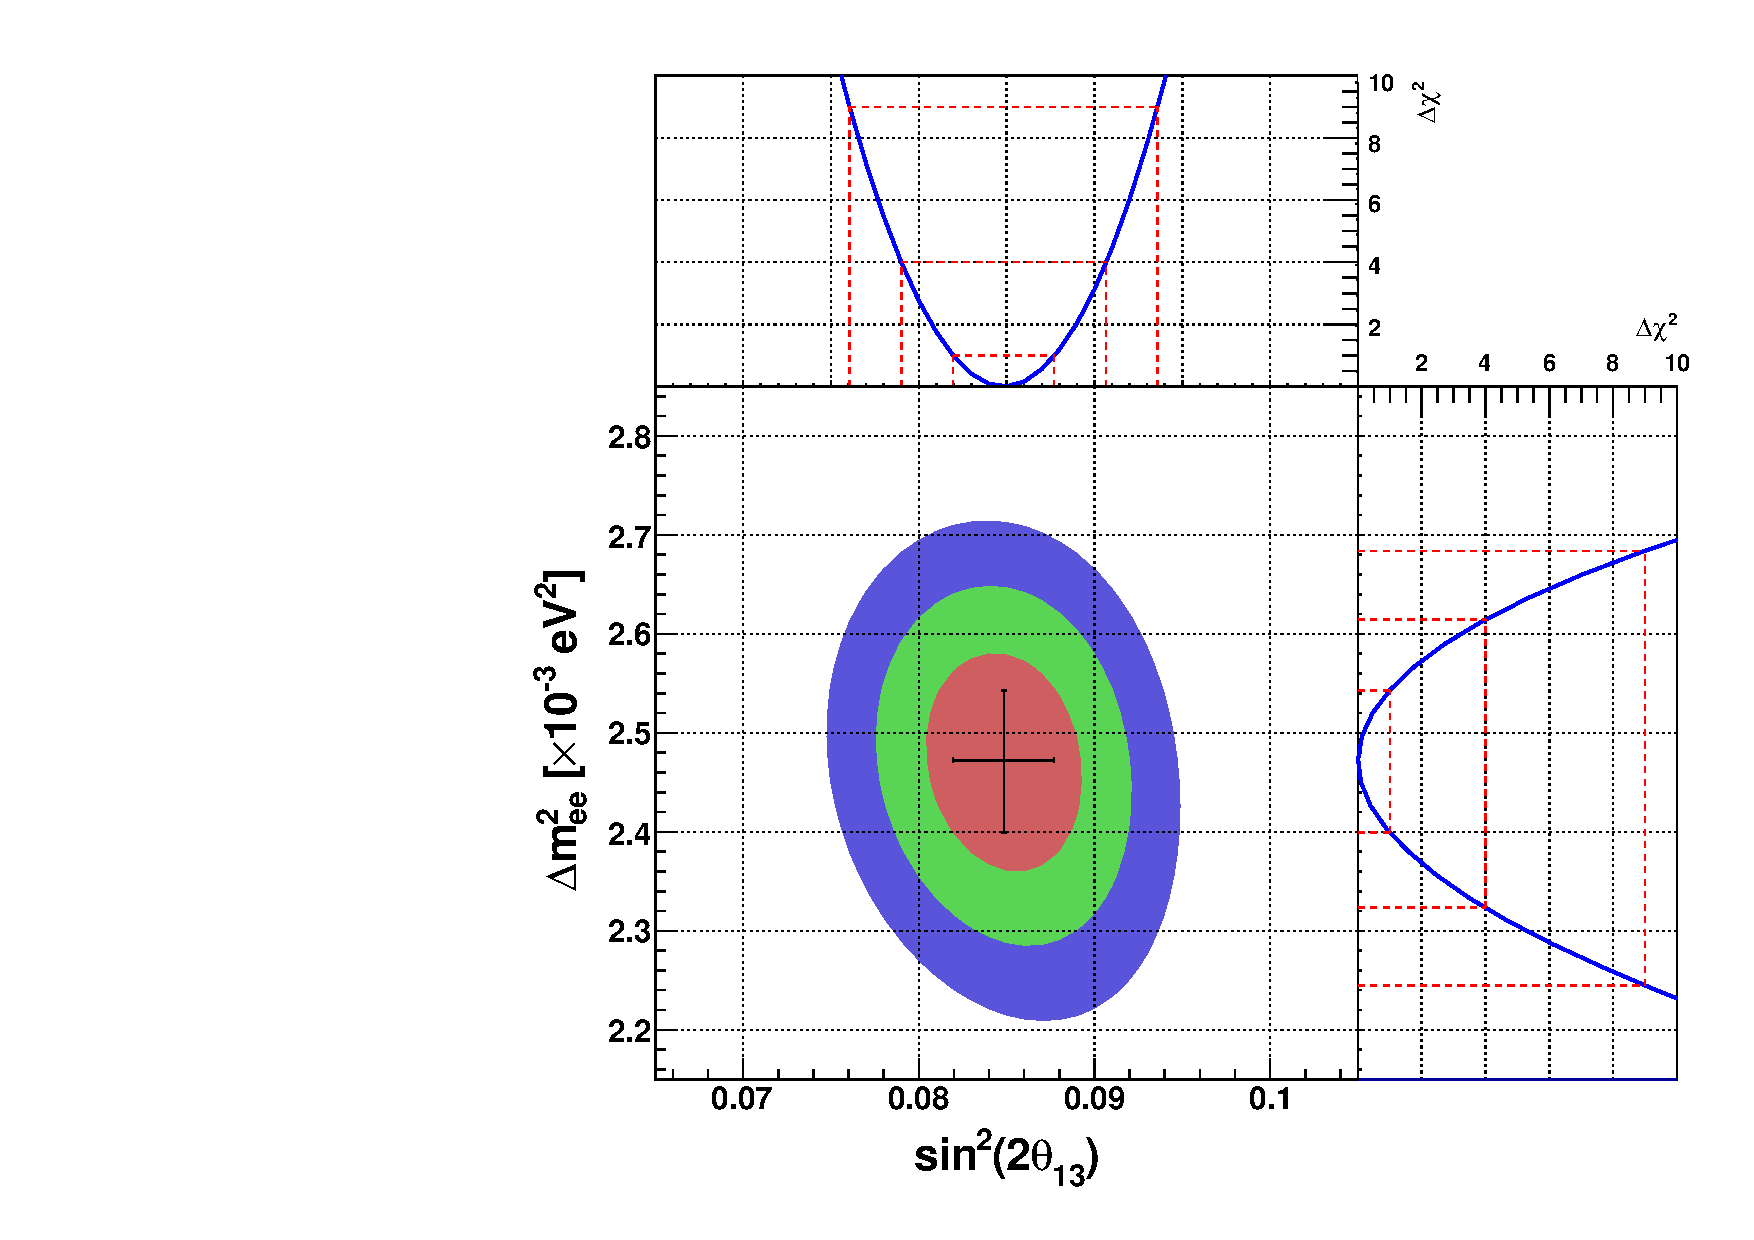
\includegraphics[scale=0.5]{Fitting/contour_Matt.pdf}
  \caption{68\%, 95\%, and 99\% C.L.\@ contours obtained from running the fitter on our IBD sample. The black cross is the best-fit point.}
  \label{fig:fitContours}
\end{figure}


\end{document}
